\section{Периодическая система химических элементов. Структура таблицы Д.И. Менделеева, группы, периоды и блоки. Металлы и неметаллы.}

\Def{Периодический закон}

Свойства химических элементов, а также формы и свойства образуемых ими простых веществ и соединений, находятся в периодической зависимости от величины зарядов ядер их атомов.

\subsection{Периодическая таблица}

\begin{figure}[H]
    \centering
    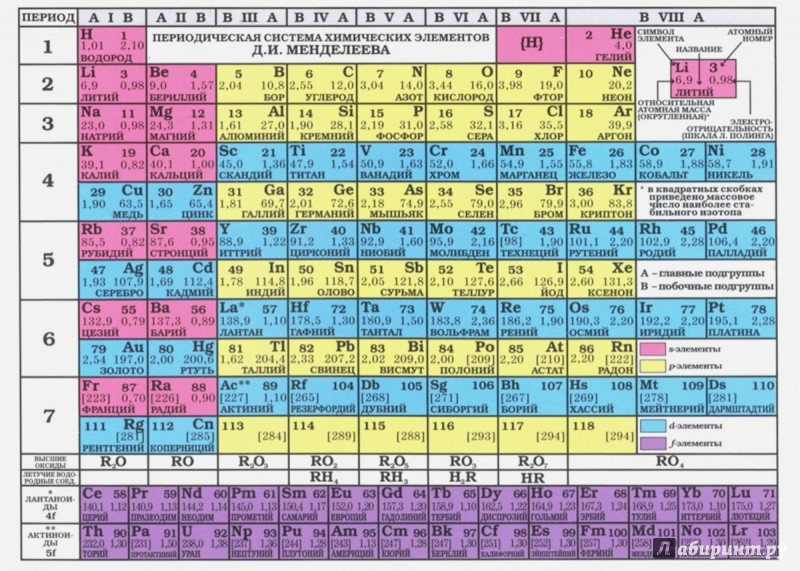
\includegraphics[width = \textwidth]{TeX/Pictures/2_table.jpg}
    \caption{Периодическая таблица Менделеева: краткая форма}
    \label{fig:table}
\end{figure}

\subsection{Структура}
\Def{Период}

Ряд в таблице Менделеева; последовательность элементов, начинающаяся щелочным металлом (или водородом) и заканчивающаяся инертным газом. 

В направлении «слева направо» атомный радиус обычно сокращается (в силу того, что у каждого последующего элемента увеличивается количество заряженных частиц, и электроны притягиваются ближе к ядру), и параллельно с ним возрастает энергия ионизации и электроотрицательность.

\Def{Группа}

Столбец в таблице Менделеева. 

Высшая степень окисления равна номеру группы со знаком «плюс». Низшая определяется, как номер группы минус 8.

Элементы одной группы проявляют схожие свойства, поэтому группы часто имеют особые названия:

\begin{table}[H]
    \centering
    \begin{tabular}{c|c}
    \hline
        Номер группы (подгруппы) &  Название\\
         1 (кроме H) &  Щелочные металлы \\
         2 (кроме Mg, Be) &  Щелочноземельные металлы \\
         16 &  Халькогены \\
         17 &  Галогены \\
         18 &  Инертные газы \\
    \hline
    \end{tabular}
    \caption{Названия некоторых групп периодической системы}
    \label{tab:groups}
\end{table}

 По направлению сверху вниз в рамках группы радиус атома возрастает (чем больше у него заполненных энергетических уровней, тем дальше от ядра располагаются валентные электроны), а энергия ионизации и электроотрицательность снижается (связи в атоме ослабевают, и, следовательно, изъять электрон становится проще).
 
 \Def{Блоки}
 
 Деление в соответствии с оболочкой, на которой находится последний электрон.
 
 \begin{figure}[H]
     \centering
     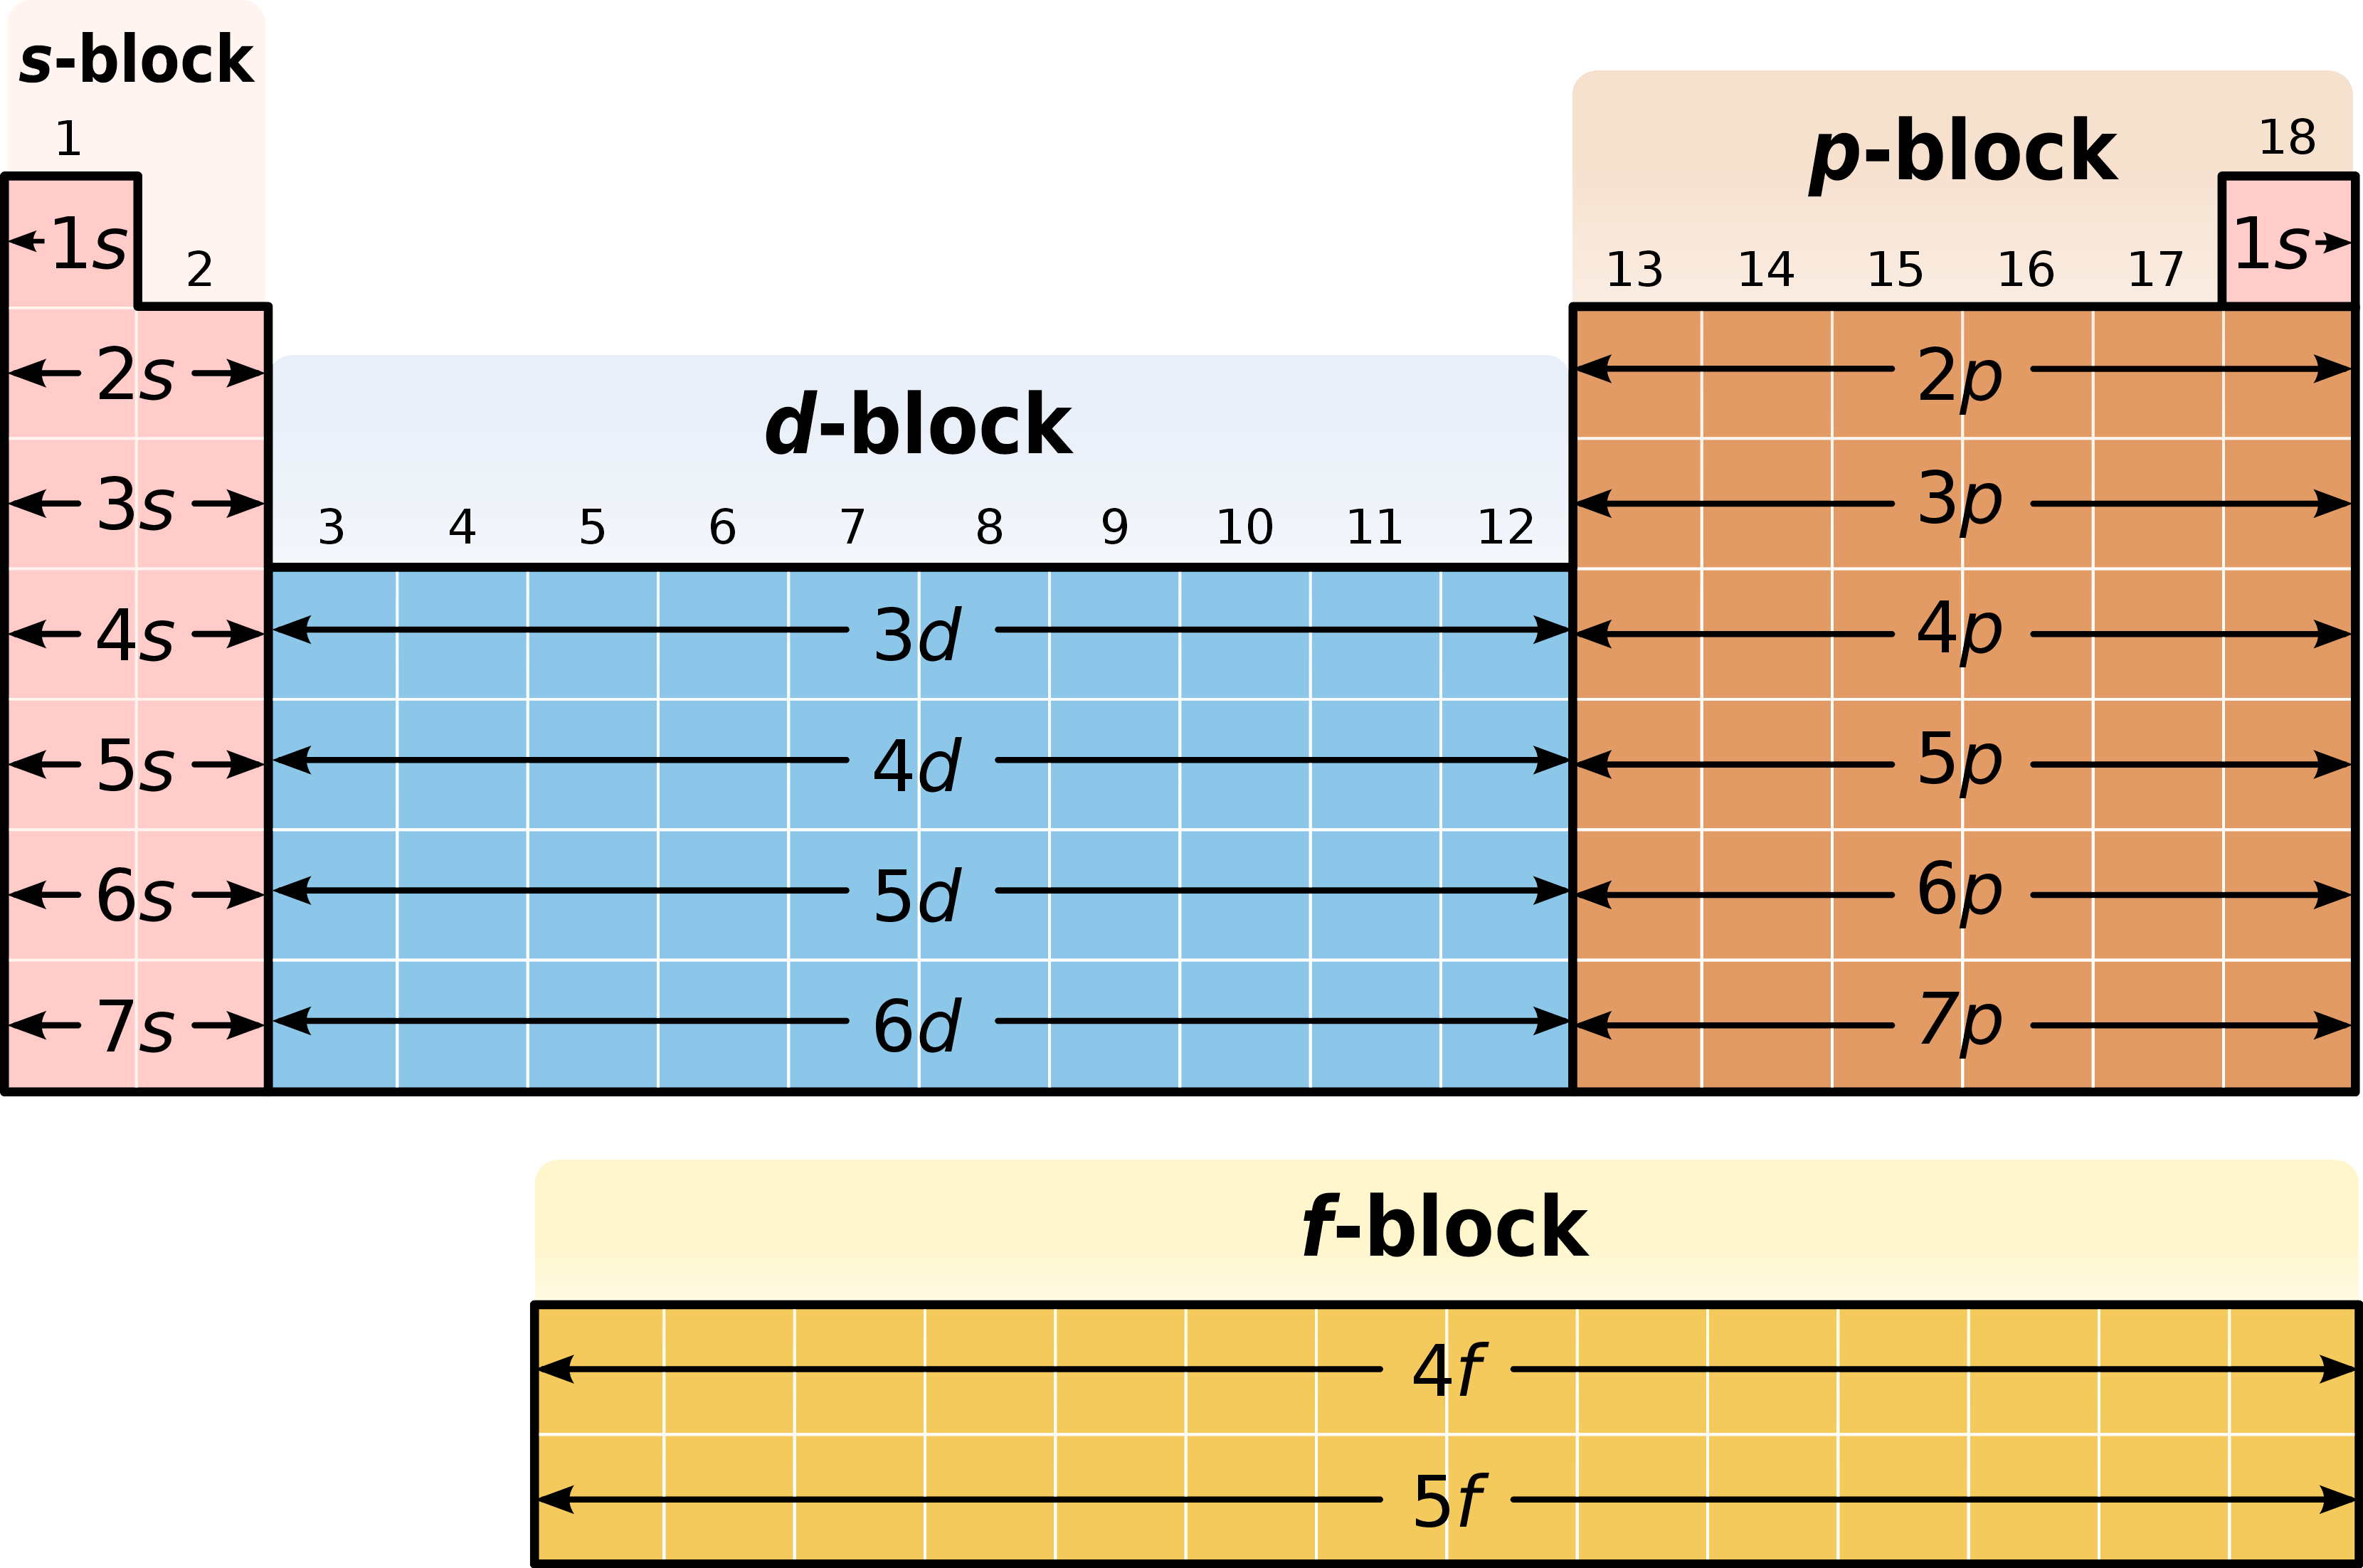
\includegraphics[width = \textwidth]{TeX/Pictures/2_block.png}
     \caption{Деление на блоки}
     \label{fig:block}
 \end{figure}
 
 \subsection{Металлы и неметаллы}
 
Традиционно деление на 2 группы: металлы имеют высокую тепло- и электропроводность, положительный температурный коэффициент сопротивления, высокую пластичность, ковкость и металлический блеск; неметаллы же определяют большая способность к присоединению дополнительных электронов, и проявление более высокой окислительной активности, чем у металлов.

\begin{figure}[H]
    \centering
    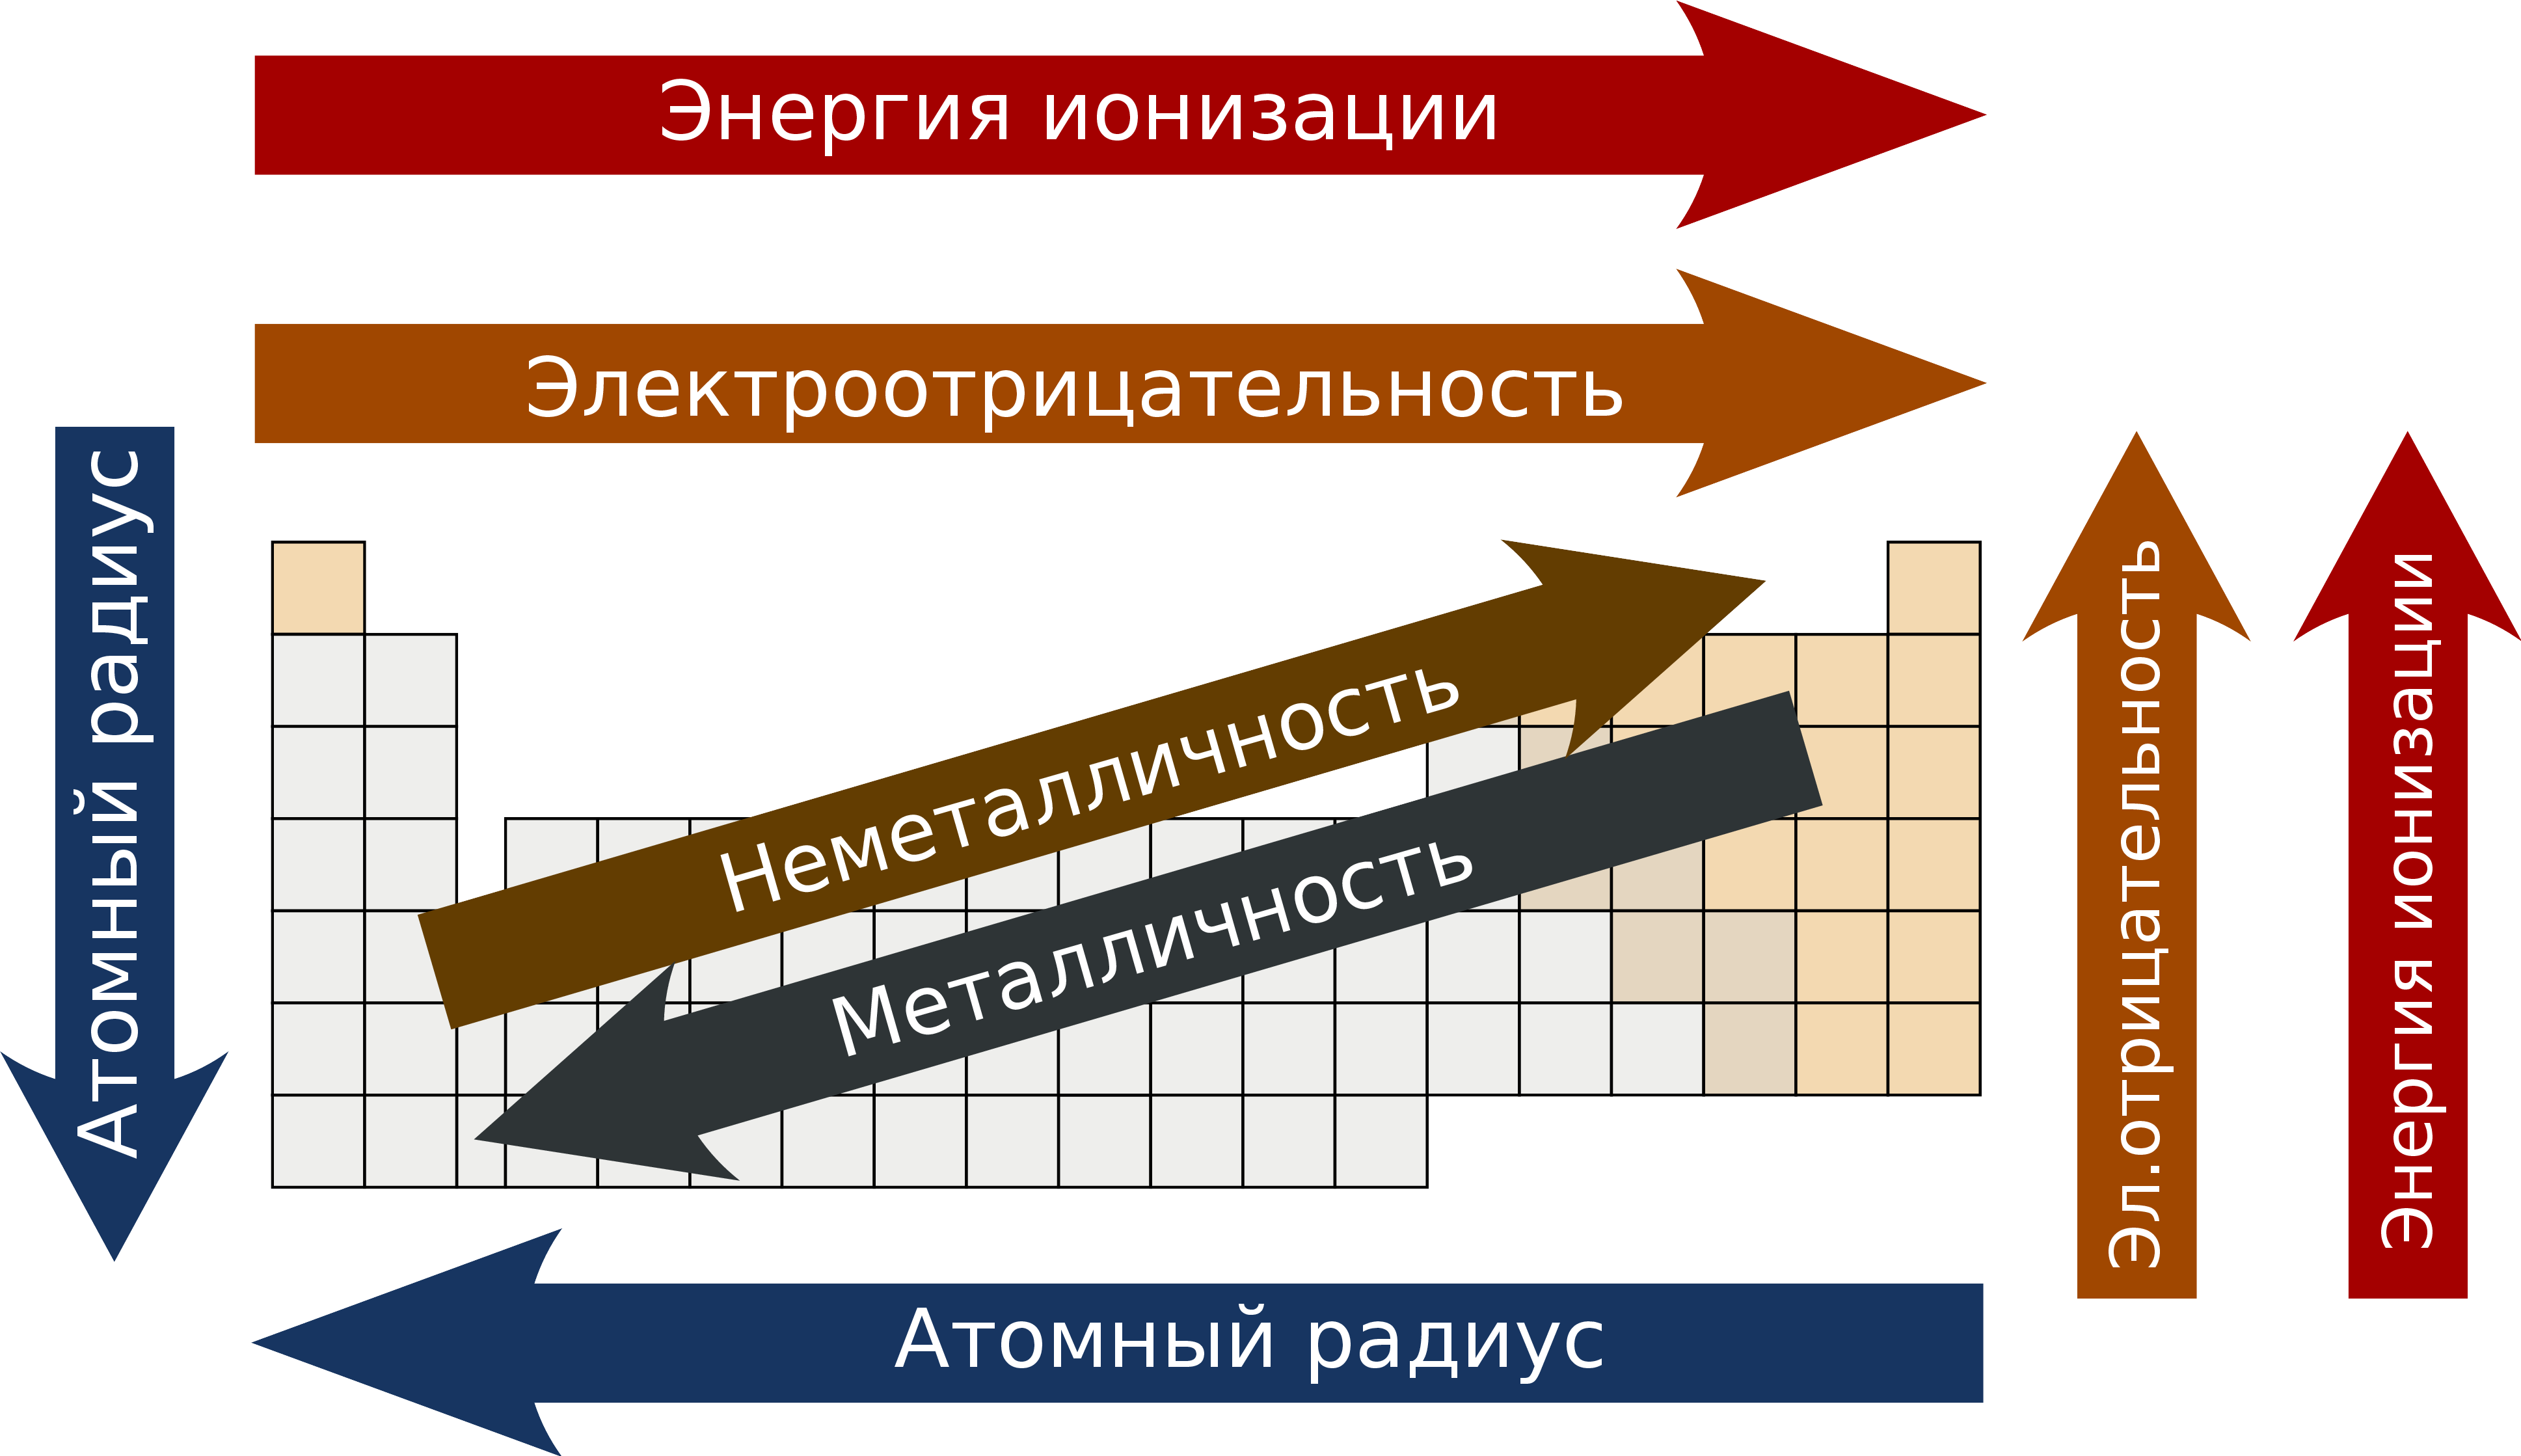
\includegraphics[width = \textwidth]{TeX/Pictures/2_properties.png}
    \caption{Свойства элементов}
    \label{fig:properties}
\end{figure}

Металлы, взаимодействуя с неметаллами, чаще образуют ионные соединения:

\ce{2 Na + Cl_2 = 2 NaCl}

Металлы, взаимодействуя друг с другом, образуют сплавы, обладающими всеми свойствами чистых металлов.

Неметаллы, взаимодействуя друг с другом, часто образуют летучие соединения с молекулярной связью:

\ce{2P+3Cl_2=2PCl_3}

